% !TEX program = xelatex
\documentclass[a4paper,11.5pt,UTF8]{ctexart}
\usepackage{a4}
\usepackage{amsmath, amssymb, amsthm, graphicx, xspace,array,url}
\usepackage{booktabs}
\usepackage{caption}
\usepackage{subcaption}
\usepackage{setspace}
\usepackage{float}
\usepackage{listings,color,xcolor,fontspec}

\CTEXsetup[format={\Large\bfseries}]{section}

\author{张卓涵 3190101161}
\usepackage[a4paper,left=20mm,right=20mm,top=30mm,bottom=20mm]{geometry}

\newtheorem{example}{\hspace{2em}例}{}
\newtheorem{remark}{\hspace{2em}注}{}
\newtheorem{thm}{\hspace{2em}定理}{}
\newtheorem{lemma}{\hspace{2em}引理}{}

\lstset{
	columns=fixed,       
	% numbers=left,
	% numberstyle=\tiny\color{gray},
	frame=lrtb,
	basicstyle=\ttfamily, 
	backgroundcolor=\color[RGB]{245,245,244},
	keywordstyle=\color[RGB]{40,40,255},
	numberstyle=\footnotesize\color{darkgray},           
	commentstyle=\it\color[RGB]{0,96,96},
	stringstyle=\rmfamily\slshape\color[RGB]{128,0,0},
	showstringspaces=false,
	language=c++,
}

\begin{document}
\begin{figure}[t]
\begin{minipage}[h]{0.25\linewidth}
	
\includegraphics[width=4.0cm]{./image/ZJU2.jpeg}
\end{minipage}
\hfill
\begin{minipage}[h]{.7\linewidth}
	\begin{flushright}
			\Large{微分方程数值解
				\vspace{3mm}	\\
				   2022 夏
				\vspace{3mm}	\\
				   张卓涵 \hspace{3mm}3190101161}
	\end{flushright}
\end{minipage}
\rule{\linewidth}{0.1em}
\end{figure}
\begin{center}
	\huge{\textbf{Project 3}}
\end{center}
\begin{large}

\section{Design Description}
\par 本次作业的程序中,依靠Vec.h文件中定义的向量类,通过类继承的方法实现了要求中的各种IVP数值方法。
\subsection{Base Class: TimeIntegrator}
\par TimeIntegrator作为抽象基类,以维度dim作为模板参数,求解的数值结果作为其成员变量,并在其中定义了若干格式化输出函数,以便测试和绘图。
\begin{lstlisting}
template<int dim>
class TimeIntegrator
{
public:
    void display() const;
    void disp_for_matplot() const;
    friend std::ostream& operator<<(std::ostream &os,
                                TimeIntegrator<dim> &TI);
    virtual Vec<real,dim> solve(const Vec<real,dim> &U0, Func f, 
                                    real T, int p_=0) const = 0;
    virtual real solution_error(const Vec<real,dim> &U0, Func f, 
                                          real T, int p_=0) = 0;
protected:
    mutable std::vector<Vec<real,dim>> result_;
}
\end{lstlisting}
其中,solve()函数包含一个提供了默认值的参数p\_,这是因为有些方法需要指定收敛阶,考虑到程序主体需要采用对象工厂的方式调用,因此其构造函数的参数列表是如一的,所以考虑两种方式:1.将p作为构造函数的提供默认值参数,即p是需要指定收敛阶的方法的成员;2.将p作为solve()函数的提供默认值参数。这里采用第二种思路,这样构造出来的方法更灵活,能够使用同一个实例对象针对不同问题采用不同的收敛阶计算,而无需再去生成一个。

\subsection{Inherited Classes: Numerical Methods}
\par 其余方法由基类继承而来,在这些方法里实现了虚函数solve()和solution\_error()用于调用相应算法求解和计算误差。其中在多数算法中solution\_error()函数采用Richardson etrapolation的粗略弱化版本,即将步长调整为原步长的一半后求解作为准确值以求误差,在forward Euler方法中则是采用Definition 10.229中的原Richardson extrapolation算法计算误差。 
\par 此外在每个继承类中增加了一个成员变量
\begin{lstlisting}
private:
    int steps_;
\end{lstlisting}
用于记录总步数。之所以没有把steps\_变量直接作为基类的成员变量由继承类继承,是因为对于自适应步长算法,步数不是固定的,所以并不需要一个固定的步数作为其成员。不过在实际的Fehlberg 4(5)算法和Dormand-Prince 5(4)算法中仍然提供了这样一个成员变量steps\_,这里是为了给算法设定一个初始步长,即使用$k=\text{T}/\text{steps\_}$作为算法的初始步长。
\par 在一些隐式方法中,在求解非线性方程组时,考虑到求解的实际上是方程$f$的不动点,所以我直接采用了最简单的不动点迭代的形式,即$x_{k+1}=f(x_k)$,只需要保证初始点$x_0$与所求不动点$x$足够接近即可。这里我在每次迭代求$U^{n+1}$时都把初始点设置为已知的$U^n$,这样在步长$k$足够小时就能保证初始点充分的接近不动点。实际在测试中,这个迭代过程的效果也是不错的。

\section{Tests}
\par 为了不使篇幅过于冗长,下面只展示部分数值结果,完整结果可见于output目录下的txt文件中。在以下测试中,(10.199)的误差显著小于(10.198),这是因为(10.198)中的精确解是给定的,而(10.199)中的“精确解”是通过算法提高精度算出来的,所以在计算出的(10.199)问题的误差会明显更小。
\subsection{Adams-Bashforth}
\begin{center}
\begin{tabular}{|c|c|c|c|c|}
    \hline
     & \multicolumn{2}{c|}{(10.198) with $T_1$ and $p=4$} & \multicolumn{2}{c|}{(10.199) with $T_2$ and $p=4$} \\
     \hline
     steps & solution error & CPU time (s) & solution error & CPU time (s) \\
     \hline
     100000 & 0.21655 & 0.265623 & 3.65037e-06 & 0.203932 \\
     \hline
     200000 & 0.0162245 & 0.516608 & 4.56275e-07 & 0.40101 \\
     \hline
     400000 & 0.000895183 & 1.04227 & 5.70457e-08 & 0.775189 \\
     \hline
\end{tabular}
\end{center}
\par 可以看到,对于(10.198),随着步数的增加一倍,其误差基本上是缩小为原来的$\frac{1}{16}$,即基本是4阶收敛的,符合预期。对于(10.199),随着步数增加一倍,误差基本上缩小为原来的$\frac{1}{8}$,即基本是3阶收敛的,符合预期。
\par 但是这里步数直到达到$10^5$的数量级才得到比较好的结果和收敛性,运行时间也一度接近甚至超过1秒,所以Adams-Bashforth算法在这个例子下是比较低效的。

\subsection{Adams-Moulton}
\begin{center}
\begin{tabular}{|c|c|c|c|c|}
    \hline
     & \multicolumn{2}{c|}{(10.198) with $T_1$ and $p=3$} & \multicolumn{2}{c|}{(10.199) with $T_2$ and $p=3$} \\
     \hline
     steps & solution error & CPU time (s) & solution error & CPU time (s) \\
     \hline
     100000 & 0.0246602 & 0.388896 & 4.05709e-07 & 0.381835 \\
     \hline
     200000 & 0.00499744 & 0.769632 & 5.0706e-08 & 0.767768 \\
     \hline
     400000 & 0.000604053 & 1.53255 & 6.34028e-09 & 1.54895 \\
     \hline
\end{tabular}
\end{center}
\par 可以看到,对于(10.198),随着步数的增加一倍,其误差基本上是缩小为原来的$\frac{1}{8}$,即基本是3阶收敛的,符合预期。对于(10.199),随着步数增加一倍,误差基本上缩小为原来的$\frac{1}{8}$,即基本是3阶收敛的,符合预期。
\par 但是这里同样步数直到达到$10^5$的数量级才得到比较好的结果和收敛性,运行时间也比较长,所以Adams-Moulton算法在这个例子下也是比较低效的。

\subsection{Backward Differentiation Formulas}
\begin{center}
\begin{tabular}{|c|c|c|c|c|}
    \hline
     & \multicolumn{2}{c|}{(10.198) with $T_1$ and $p=4$} & \multicolumn{2}{c|}{(10.199) with $T_2$ and $p=4$} \\
     \hline
     steps & solution error & CPU time (s) & solution error & CPU time (s) \\
     \hline
     100000 & 0.0984906 & 0.27678 & 0.378463 & 0.299356 \\
     \hline
     200000 & 0.241012 & 0.560489 & 0.492389 & 0.566249 \\
     \hline
     400000 & 0.281448 & 1.10923 & 0.0287123 & 1.1252 \\
     \hline
\end{tabular}
\end{center}
\par BDF算法的运行结果是很糟糕的,即便是步数达到了$10^5$的数量级,误差也没有达到可以接受的精度,更没有收敛性。

\subsection{Classical Runge-Kutta}
\begin{center}
\begin{tabular}{|c|c|c|c|c|}
    \hline
     & \multicolumn{2}{c|}{(10.198) with $T_1$} & \multicolumn{2}{c|}{(10.199) with $T_2$} \\
     \hline
     steps & solution error & CPU time (s) & solution error & CPU time (s) \\
     \hline
     12000 & 1.76256 & 0.031874 & 2.11243e-09 & 0.031925 \\
     \hline
     24000 & 0.204469 & 0.064156 & 3.30833e-10 & 0.064365 \\
     \hline
     48000 & 0.0108932 & 0.127158 & 2.41786e-11 & 0.129579 \\
     \hline
\end{tabular}
\end{center}
\par 对于(10.198),随着步数的增加一倍,其误差基本上是缩小为原来的$\frac{1}{8}\text{到}\frac{1}{16}$,即基本可以认定符合预期的4阶收敛。对于(10.199),随着步数增加一倍,误差基本上缩小为原来的$\frac{1}{8}\text{到}\frac{1}{16}$,即基本也是4阶收敛的。
\par 从下文中的图像可以看到,经典RK方法虽然在求解(10.198)问题中的误差没有达到很小的数量级,但这个结果已经足以保证绘制出非常接近准确解的图像了。

\subsection{ESDIRK}
\begin{center}
\begin{tabular}{|c|c|c|c|c|}
    \hline
     & \multicolumn{2}{c|}{(10.198) with $T_1$} & \multicolumn{2}{c|}{(10.199) with $T_2$} \\
     \hline
     steps & solution error & CPU time (s) & solution error & CPU time (s) \\
     \hline
     10000 & 1.54671 & 0.161873 & 2.74876e-08 & 0.177303 \\
     \hline
     20000 & 0.125585 & 0.30029 & 5.16898e-09 & 0.347471 \\
     \hline
     40000 & 0.0076391 & 0.595244 & 2.44824e-09 & 0.632963 \\
     \hline
\end{tabular}
\end{center}
\par 对于(10.198),随着步数的增加一倍,其误差基本上是缩小为原来的$\frac{1}{16}$,即基本可以认定4阶收敛。对于(10.199),步数从10000到20000的过程中满足4阶的收敛率,在20000到40000的过程中,误差下降很少,推断是因为两个问题计算误差的方法不同,(10.199)中的“精确解”实际上是采用更准确的方法得到的数值解,所以在步长充分小的时候,误差的下降是越来越慢的。

\subsection{Gauss-Legendre RK}
\begin{center}
\begin{tabular}{|c|c|c|c|c|}
    \hline
     & \multicolumn{2}{c|}{(10.198) with $T_1$ and $s=2$} & \multicolumn{2}{c|}{(10.199) with $T_2$ and $s=1$} \\
     \hline
     steps & solution error & CPU time (s) & solution error & CPU time (s) \\
     \hline
     10000 & 1.18123 & 0.065197 & 0.00101314 & 0.032234 \\
     \hline
     20000 & 0.0796395 & 0.135682 & 0.00025186 & 0.061937 \\
     \hline
     40000 & 0.0051198 & 0.263749 & 5.69224e-05 & 0.117864 \\
     \hline
\end{tabular}
\end{center}
\par 对于(10.198),随着步数的增加一倍,其误差基本上是缩小为原来的$\frac{1}{16}$,即基本可以认定为符合预期的4阶收敛。对于(10.199),随着步数的增加一倍,其误差基本上是缩小为原来的$\frac{1}{4}$,即基本可以认定为符合预期的2阶收敛。

\subsection{Fehlberg 4(5) embedded RK}
\begin{center}
\begin{tabular}{|c|c|c|c|c|}
    \hline
     & \multicolumn{2}{c|}{(10.198) with $T_1$} & \multicolumn{2}{c|}{(10.199) with $T_2$} \\
     \hline
     initial step length & solution error & CPU time (s) & solution error & CPU time (s) \\
     \hline
     0.01 & 0.0145282 & 0.002217 &  & 0.002722 \\
     \hline
\end{tabular}
\end{center}
\par 考虑到,嵌入式RK方法是自适应步长的,所以这里不再展示收敛率和(10.199)问题的误差。事实上从下文可以看到,自适应步长方法是效果最好、效率最高的方法。

\subsection{Dormand-Prince 5(4) embedded RK}
\begin{center}
\begin{tabular}{|c|c|c|c|c|}
    \hline
     & \multicolumn{2}{c|}{(10.198) with $T_1$} & \multicolumn{2}{c|}{(10.199) with $T_2$} \\
     \hline
     initial step length & solution error & CPU time (s) & solution error & CPU time (s) \\
     \hline
     0.01 & 0.000894613 & 0.002525 &  & 0.00328 \\
     \hline
\end{tabular}
\end{center}
\par 同理,结合下文可以看到,Dorman-Prince方法显示出更小的误差和更好的效果。

\section{Plots}
\begin{itemize}
    \item Euler method with 24000 steps.
    \begin{figure}[H]
        \centering
        %\subfigure
        %{
            \begin{minipage}{0.48\textwidth}
    	    \centering
    	    \caption{(10.198) with $T_1$}
    	    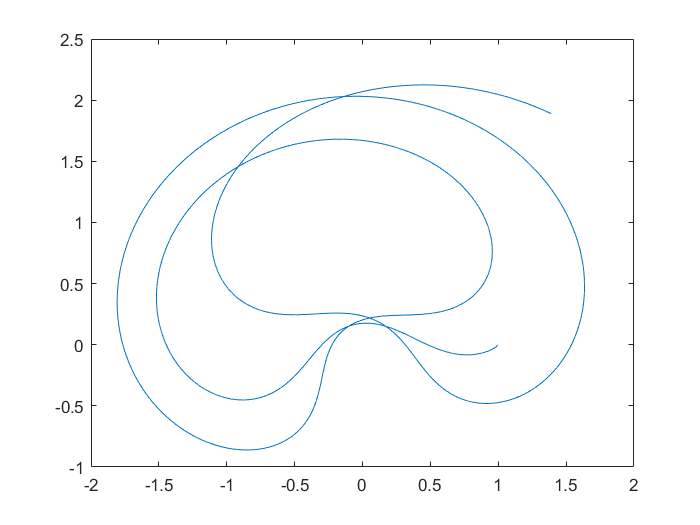
\includegraphics[scale=0.48]{./image/Euler_1.png}
    	    \end{minipage}
        %}
        %\subfigure
        %{
            \begin{minipage}{0.48\textwidth}
    	    \centering
    	    \caption{(10.199) with $T_2$}
    	    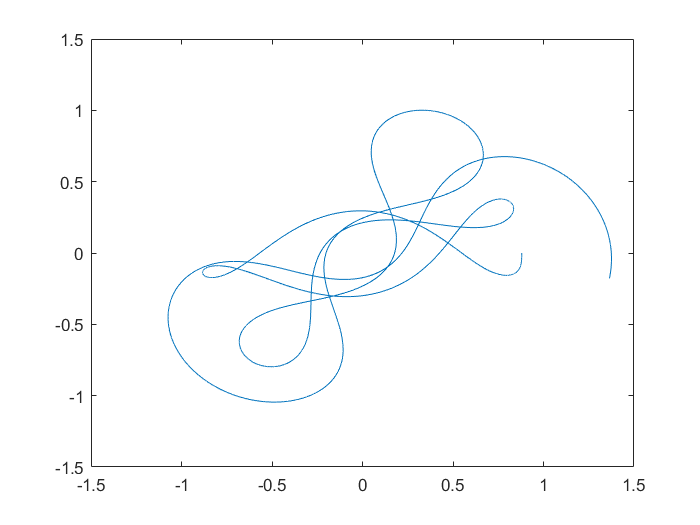
\includegraphics[scale=0.48]{./image/Euler_2.png}
    	    \end{minipage}
        %}
        \label{fig:1}
    \end{figure}
    可以看到,24000步的Euler方法得到的结果是很糟糕的,实际上,即便是步数达到$10^5$数量级,也依然不能呈现出比较好的结果。\\
    (10.198)耗时:0.046518秒;(10.199)耗时:0.016837秒。
    \item Classical RK method with 12000 steps.
    \begin{figure}[H]
        \centering
        %\subfigure
        %{
            \begin{minipage}{0.48\textwidth}
    	    \centering
    	    \caption{(10.198) with $T_1$}
    	    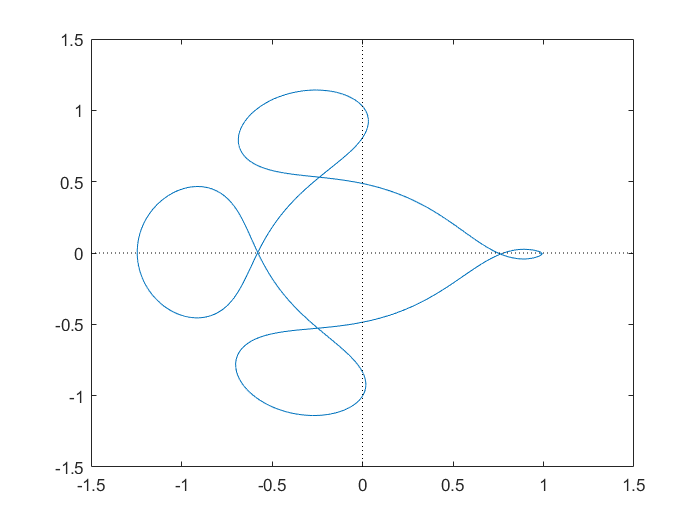
\includegraphics[scale=0.48]{./image/CRK_1.png}
    	    \end{minipage}
        %}
        %\subfigure
        %{
            \begin{minipage}{0.48\textwidth}
    	    \centering
    	    \caption{(10.199) with $T_2$}
    	    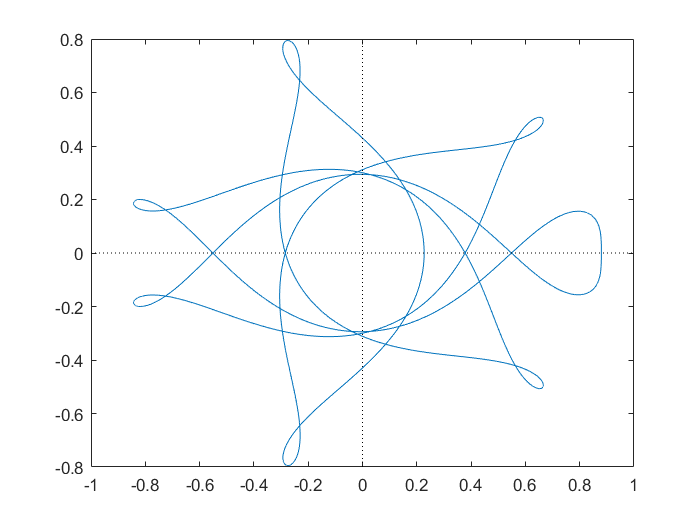
\includegraphics[scale=0.48]{./image/CRK_2.png}
    	    \end{minipage}
        %}
        \label{fig:2}
    \end{figure}
    这里,由于6000步的经典RK方法呈现的结果欠佳,将步数提高一倍就得到了非常好的结果。\\
    (10.198)耗时:0.03287秒;(10.199)耗时:0.031312秒。
    \item Dormand-Prince 5(4) method with initial step length 0.01.
    \begin{figure}[H]
        \centering
        %\subfigure
        %{
            \begin{minipage}{0.48\textwidth}
    	    \centering
    	    \caption{(10.198) with $T_1$}
    	    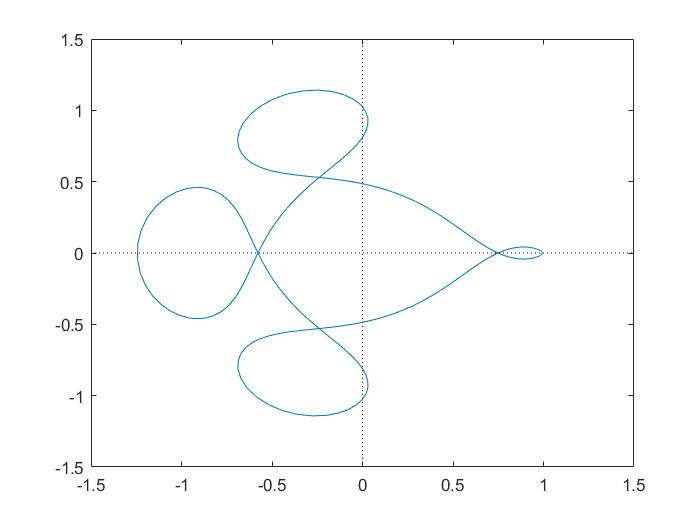
\includegraphics[scale=0.48]{./image/DP54_1.png}
    	    \end{minipage}
        %}
        %\subfigure
        %{
            \begin{minipage}{0.48\textwidth}
    	    \centering
    	    \caption{(10.199) with $T_2$}
    	    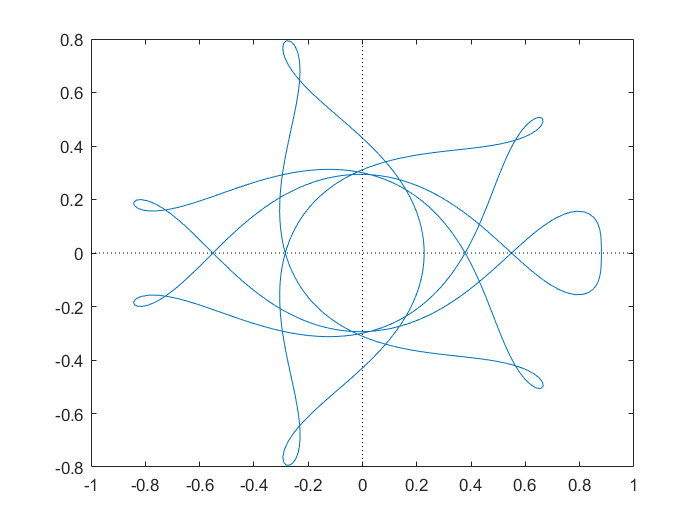
\includegraphics[scale=0.48]{./image/DP54_2.png}
    	    \end{minipage}
        %}
        \label{fig:3}
    \end{figure}
    (10.198)耗时:0.002424秒;(10.199)耗时:0.003282秒。
\end{itemize}
从上可以看到,Dormand-Prince方法耗时最短,且得到的结果最精确。

\end{large}
\end{document}